\section{Palindromo usando gramática libre de contexto}
	\subsection{Descripción del problema}
	Este problema fue parte de la introducción a las gramáticas libres de contexto o Context Free Grammars con el objetivo de generar cadenas que fueran parte del lenguaje de los palíndromos formados por ceros y unos como por ejemplo las cadenas 0011, 1111, 11011 entre otras. Dicho de otra forma, una cadena $w$ forma parte del $ L_{pal}$ si y sólo si $w=w^R$.
	Para generar el palíndromo se utilizo la siguiente GIC.\cite{LIBRO}
	\[ G_{pal} = ({P},{0,1},A,P) \]
	Donde A representa el conjunto de las siguientes 5 producciones.
	\begin{gather*}
	1. P\to \epsilon \\
	2. P\to 0 \\
	3. P\to 1 \\
	4. P\to 0P0 \\
	5. P\to 1P1
	\end{gather*}
	El programa cuenta con modo manual y automático en los cuales se introduce la longitud $0 \le n \le 1000 $ de la cadena que se desea obtener. Y se muestra el proceso de producción en pantalla y un archivo de texto.
	\subsection{Código}
	El código fue realizado en Python 3.5.
	\\Archivo: main\_palindromo.py
	\begin{lstlisting}[language=Python]
	# main_palindromo.py#
	# -*- coding: utf-8 -*-
	from __future__ import print_function
	from palindromo import palindromo
	import random

	separador = '='*50

	def main():
	    continuar = True
	    while continuar:
	        opcion = imprimir_menu()
	        if opcion == 1:
	            entrada_consola()
	        elif opcion == 2:
	            entrada_automatico()
	        else:
	            break
	        print('=' * 100)
	        opcion = input("Reintentar [s/n]: ")
	        if opcion.lower() != 's':
	            continuar = False

	    print('Saliendo del programa...')

	def imprimir_menu():
	    print("""\n\nGramatica libre de contexto Gpal = ({P},{0,1},A,P)
	    Donde A es:
	    1. P -> e
	    2. P -> 0
	    3. P -> 1
	    4. P -> 0P0
	    5. P -> 1P1
	    """)
	    print('\n%sMenu%s' % (separador, separador))
	    print("""
	        1.- Modo manual
	        2.- Modo automatico
	        4.- Salir
	    """)
	    try:
	        opcion = int(input("Selecciona una opcion valida: "))
	        return opcion
	    except Exception as e:
	        print('Error ', e)
	        return 0
	def entrada_automatico():
	    longitud = random.randint(0, 1000)
	    print("Generando palindromo con longitud = %s" % longitud)
	    palindromo(longitud)

	def entrada_consola():
	    longitud = int(input('Introduce un numero entre 0 y 1000: '))
	    if longitud>1000 or longitud<0:
	        print('Algo salio mal =(')
	        return 0
	    print("Generando palindromo con longitud = %s" % longitud)
	    palindromo(longitud)

	main()
	\end{lstlisting}
	Archivo: palindromo.py
	\begin{lstlisting}[language=Python]
	# palindromo.py
	# -*- coding: utf-8 -*-
	from __future__ import print_function
	import random
	def palindromo(repeticiones):
	    archivo = open('palindromo-historia.txt', 'w')
	    cadena = 'P'
	    base_random = ''
	    archivo.write('Longitud = %s\n' %repeticiones)
	    archivo.write(cadena + '\n')
	    print(cadena)
	    if repeticiones % 2 == 1:
	        cadena = generar_cadena(cadena, (repeticiones-1)/2, archivo)
	        base_random = random.choice(['0', '1'])
	    else:
	        cadena = generar_cadena(cadena, repeticiones/2, archivo)
	    cadena = cadena.replace('P', base_random)
	    if base_random == '':
	        base_random = 'e'
	    archivo.write('Cadena final con base P=%s -> %s\n' %(base_random, cadena))
	    print('Cadena final con base P=%s -> %s' %(base_random, cadena))
	    archivo.close()

	def generar_cadena(cadena, repeticiones, archivo):
	    if repeticiones > 0:
	        regla = random.choice(['0', '1'])
	        cadena = cadena.replace('P', regla+'P'+regla)
	        print('%s    Regla usada: %sP%s ' %(cadena, regla, regla))
	        archivo.write('%s    Regla usada: %sP%s \n' %(cadena, regla, regla))
	        repeticiones = repeticiones - 1
	        cadena = generar_cadena(cadena, repeticiones, archivo)
	    return cadena
	\end{lstlisting}
	\newpage
	\subsection{Pruebas}
	Pruebas de las opciones del menú.
	\\
	{\large Modo de manual}
	\begin{figure}[H]
		\begin{center}
			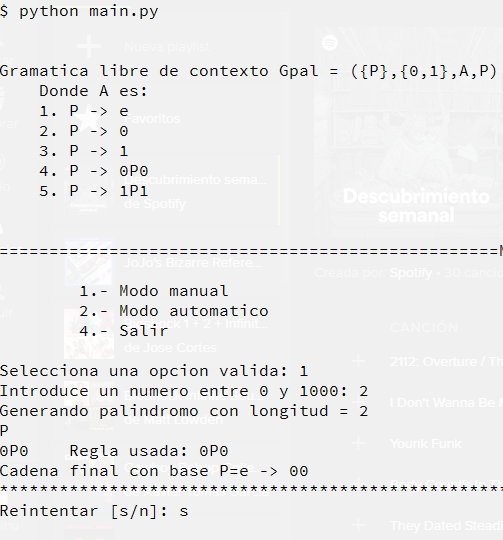
\includegraphics[width=10cm, height=8cm]{img/palindromo-manual-consola.png}
			\caption{Historia de la generación del palíndromo en consola.}
			\label{fig:palindromo1}
		\end{center}
	\end{figure}
	\begin{figure}[H]
		\begin{center}
			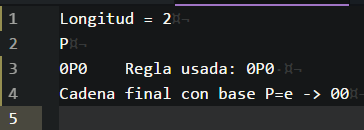
\includegraphics[width=10cm, height=5cm]{img/palindromo-manual-archivo.png}
			\caption{Historia de la generación del palíndromo en archivo.}
			\label{fig:palindromo2}
		\end{center}
	\end{figure}
	\newpage
	{\large Modo de automático}
	\begin{figure}[H]
		\begin{center}
			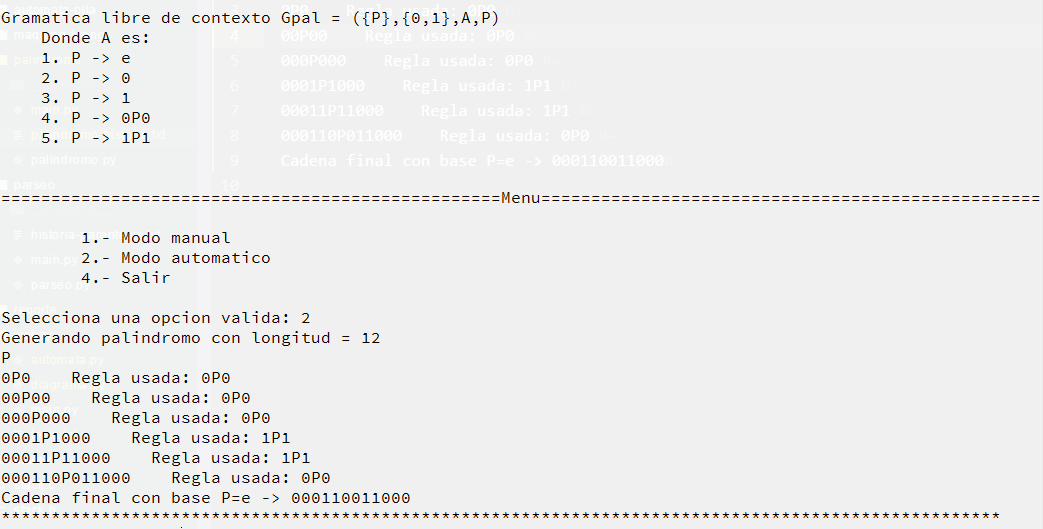
\includegraphics[width=\linewidth, height=8cm]{img/palindromo-automatico-consola.png}
			\caption{Historia de la generación del palíndromo en consola.}
			\label{fig:palindromo3}
		\end{center}
	\end{figure}
	\begin{figure}[H]
		\begin{center}
			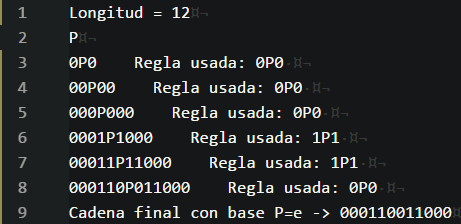
\includegraphics[width=\linewidth, height=8cm]{img/palindromo-automatico-archivo.png}
			\caption{Historia de la generación del palindromo en archivo.}
			\label{fig:palindromo4}
		\end{center}
	\end{figure}
